\documentclass[twoside]{book}

% Packages required by doxygen
\usepackage{calc}
\usepackage{doxygen}
\usepackage{graphicx}
\usepackage[utf8]{inputenc}
\usepackage{makeidx}
\usepackage{multicol}
\usepackage{multirow}
\usepackage{textcomp}
\usepackage[table]{xcolor}

% Font selection
\usepackage[T1]{fontenc}
\usepackage{mathptmx}
\usepackage[scaled=.90]{helvet}
\usepackage{courier}
\usepackage{amssymb}
\usepackage{sectsty}
\renewcommand{\familydefault}{\sfdefault}
\allsectionsfont{%
  \fontseries{bc}\selectfont%
  \color{darkgray}%
}
\renewcommand{\DoxyLabelFont}{%
  \fontseries{bc}\selectfont%
  \color{darkgray}%
}

% Page & text layout
\usepackage{geometry}
\geometry{%
  a4paper,%
  top=2.5cm,%
  bottom=2.5cm,%
  left=2.5cm,%
  right=2.5cm%
}
\tolerance=750
\hfuzz=15pt
\hbadness=750
\setlength{\emergencystretch}{15pt}
\setlength{\parindent}{0cm}
\setlength{\parskip}{0.2cm}
\makeatletter
\renewcommand{\paragraph}{%
  \@startsection{paragraph}{4}{0ex}{-1.0ex}{1.0ex}{%
    \normalfont\normalsize\bfseries\SS@parafont%
  }%
}
\renewcommand{\subparagraph}{%
  \@startsection{subparagraph}{5}{0ex}{-1.0ex}{1.0ex}{%
    \normalfont\normalsize\bfseries\SS@subparafont%
  }%
}
\makeatother

% Headers & footers
\usepackage{fancyhdr}
\pagestyle{fancyplain}
\fancyhead[LE]{\fancyplain{}{\bfseries\thepage}}
\fancyhead[CE]{\fancyplain{}{}}
\fancyhead[RE]{\fancyplain{}{\bfseries\leftmark}}
\fancyhead[LO]{\fancyplain{}{\bfseries\rightmark}}
\fancyhead[CO]{\fancyplain{}{}}
\fancyhead[RO]{\fancyplain{}{\bfseries\thepage}}
\fancyfoot[LE]{\fancyplain{}{}}
\fancyfoot[CE]{\fancyplain{}{}}
\fancyfoot[RE]{\fancyplain{}{\bfseries\scriptsize Generated on Thu Aug 15 2013 13:02:16 by Doxygen }}
\fancyfoot[LO]{\fancyplain{}{\bfseries\scriptsize Generated on Thu Aug 15 2013 13:02:16 by Doxygen }}
\fancyfoot[CO]{\fancyplain{}{}}
\fancyfoot[RO]{\fancyplain{}{}}
\renewcommand{\footrulewidth}{0.4pt}
\renewcommand{\chaptermark}[1]{%
  \markboth{#1}{}%
}
\renewcommand{\sectionmark}[1]{%
  \markright{\thesection\ #1}%
}

% Indices & bibliography
\usepackage{natbib}
\usepackage[titles]{tocloft}
\setcounter{tocdepth}{3}
\setcounter{secnumdepth}{5}
\makeindex

% Hyperlinks (required, but should be loaded last)
\usepackage{ifpdf}
\ifpdf
  \usepackage[pdftex,pagebackref=true]{hyperref}
\else
  \usepackage[ps2pdf,pagebackref=true]{hyperref}
\fi
\hypersetup{%
  colorlinks=true,%
  linkcolor=blue,%
  citecolor=blue,%
  unicode%
}

% Custom commands
\newcommand{\clearemptydoublepage}{%
  \newpage{\pagestyle{empty}\cleardoublepage}%
}


%===== C O N T E N T S =====

\begin{document}

% Titlepage & ToC
\hypersetup{pageanchor=false}
\pagenumbering{roman}
\begin{titlepage}
\vspace*{7cm}
\begin{center}%
{\Large Reference Manual}\\
\vspace*{1cm}
{\large Generated by Doxygen 1.8.4}\\
\vspace*{0.5cm}
{\small Thu Aug 15 2013 13:02:16}\\
\end{center}
\end{titlepage}
\clearemptydoublepage
\tableofcontents
\clearemptydoublepage
\pagenumbering{arabic}
\hypersetup{pageanchor=true}

%--- Begin generated contents ---
\chapter{Hierarchical Index}
\section{Class Hierarchy}
This inheritance list is sorted roughly, but not completely, alphabetically\-:\begin{DoxyCompactList}
\item \contentsline{section}{com.\-server.\-Handle\-U\-D\-P}{\pageref{classcom_1_1server_1_1HandleUDP}}{}
\item \contentsline{section}{com.\-server.\-Server}{\pageref{classcom_1_1server_1_1Server}}{}
\item \contentsline{section}{com.\-server.\-Server\-Handler}{\pageref{classcom_1_1server_1_1ServerHandler}}{}
\item \contentsline{section}{com.\-server.\-Server\-Thread}{\pageref{classcom_1_1server_1_1ServerThread}}{}
\item Thread\begin{DoxyCompactList}
\item \contentsline{section}{com.\-server.\-Handle\-H\-T\-T\-P}{\pageref{classcom_1_1server_1_1HandleHTTP}}{}
\item \contentsline{section}{com.\-server.\-Handle\-T\-C\-P}{\pageref{classcom_1_1server_1_1HandleTCP}}{}
\end{DoxyCompactList}
\end{DoxyCompactList}

\chapter{Class Index}
\section{Class List}
Here are the classes, structs, unions and interfaces with brief descriptions\-:\begin{DoxyCompactList}
\item\contentsline{section}{\hyperlink{classcom_1_1server_1_1HandleHTTP}{com.\-server.\-Handle\-H\-T\-T\-P} \\*Class Handle\-Http This class is for handling the specific Http protocol, both P\-O\-S\-T and G\-E\-T }{\pageref{classcom_1_1server_1_1HandleHTTP}}{}
\item\contentsline{section}{\hyperlink{classcom_1_1server_1_1HandleTCP}{com.\-server.\-Handle\-T\-C\-P} \\*This class to manage upload and download requests via T\-C\-P }{\pageref{classcom_1_1server_1_1HandleTCP}}{}
\item\contentsline{section}{\hyperlink{classcom_1_1server_1_1HandleUDP}{com.\-server.\-Handle\-U\-D\-P} \\*This class handles most the primary U\-D\-P Upload and Download functionality for the server }{\pageref{classcom_1_1server_1_1HandleUDP}}{}
\item\contentsline{section}{\hyperlink{classcom_1_1server_1_1Server}{com.\-server.\-Server} \\*This class acts as the basic port handler, and contains the primary server loop }{\pageref{classcom_1_1server_1_1Server}}{}
\item\contentsline{section}{\hyperlink{classcom_1_1server_1_1ServerHandler}{com.\-server.\-Server\-Handler} \\*This class is the entry point into the program where the main method lives }{\pageref{classcom_1_1server_1_1ServerHandler}}{}
\item\contentsline{section}{\hyperlink{classcom_1_1server_1_1ServerThread}{com.\-server.\-Server\-Thread} \\*This class is the class that checks the clients local port, and hands off threads accordingly }{\pageref{classcom_1_1server_1_1ServerThread}}{}
\end{DoxyCompactList}

\chapter{Class Documentation}
\hypertarget{classcom_1_1server_1_1HandleHTTP}{\section{com.\-server.\-Handle\-H\-T\-T\-P Class Reference}
\label{classcom_1_1server_1_1HandleHTTP}\index{com.\-server.\-Handle\-H\-T\-T\-P@{com.\-server.\-Handle\-H\-T\-T\-P}}
}


class Handle\-Http This class is for handling the specific Http protocol, both P\-O\-S\-T and G\-E\-T.  


Inheritance diagram for com.\-server.\-Handle\-H\-T\-T\-P\-:\begin{figure}[H]
\begin{center}
\leavevmode
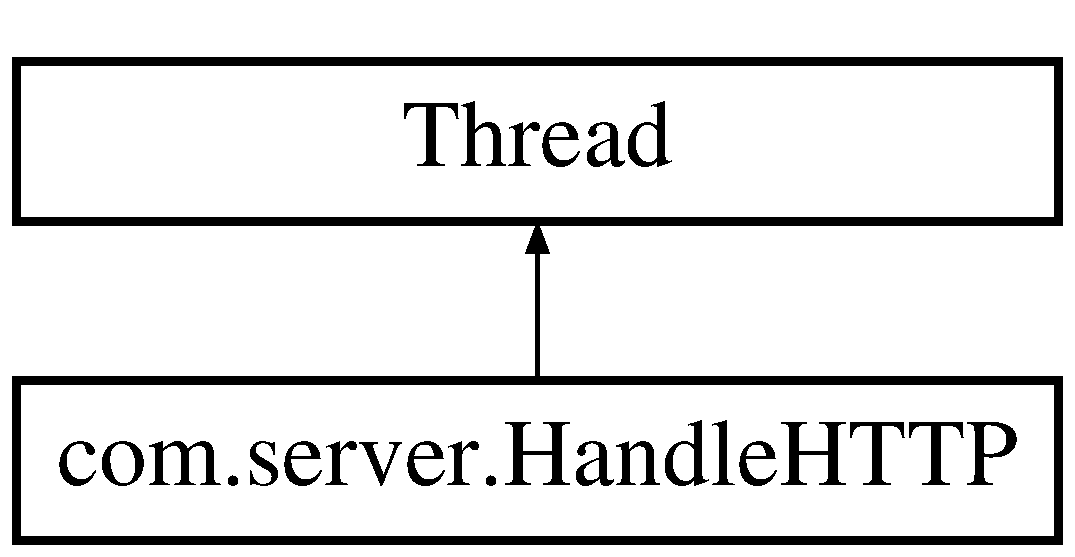
\includegraphics[height=2.000000cm]{classcom_1_1server_1_1HandleHTTP}
\end{center}
\end{figure}
\subsection*{Public Member Functions}
\begin{DoxyCompactItemize}
\item 
\hyperlink{classcom_1_1server_1_1HandleHTTP_ab3c8c02165c7be1eb515ec8311409499}{Handle\-H\-T\-T\-P} (Socket client)
\begin{DoxyCompactList}\small\item\em The only constructor, requires you have a client. \end{DoxyCompactList}\item 
\hypertarget{classcom_1_1server_1_1HandleHTTP_a016efaa23359d95eabc8fae5996c4a93}{void \hyperlink{classcom_1_1server_1_1HandleHTTP_a016efaa23359d95eabc8fae5996c4a93}{run} ()}\label{classcom_1_1server_1_1HandleHTTP_a016efaa23359d95eabc8fae5996c4a93}

\begin{DoxyCompactList}\small\item\em The main method that breaks down all of the client input string (G\-E\-T request, etc.) \end{DoxyCompactList}\item 
void \hyperlink{classcom_1_1server_1_1HandleHTTP_af21b586545963aa09597b1b23bc4d728}{data\-Dump} (Data\-Output\-Stream out)  throws I\-O\-Exception 
\begin{DoxyCompactList}\small\item\em Dumps 100 M\-B of data onto the client as fast as possible. \end{DoxyCompactList}\item 
void \hyperlink{classcom_1_1server_1_1HandleHTTP_aa8b146dea927cfd479a2866706f586e0}{black\-Hole} (Input\-Stream ins, Data\-Output\-Stream out)  throws I\-O\-Exception
\begin{DoxyCompactList}\small\item\em This method acts as the 'black hole' when a client P\-O\-S\-T\-S to the server It's assumed that the client will send as much data as it can, as fast as possible. \end{DoxyCompactList}\item 
void \hyperlink{classcom_1_1server_1_1HandleHTTP_a0f68531fee6c43a46cb461056bd01bb3}{ping\-Test} (Data\-Output\-Stream out)  throws I\-O\-Exception     
\begin{DoxyCompactList}\small\item\em This method is specifically for testing the ping from a client. \end{DoxyCompactList}\end{DoxyCompactItemize}
\subsection*{Public Attributes}
\begin{DoxyCompactItemize}
\item 
\hypertarget{classcom_1_1server_1_1HandleHTTP_a8e81d6717697e6da66f2380a5028d9bf}{Map$<$ String, String $>$ {\bfseries header\-Key\-Pair} = new Hash\-Map$<$String,String$>$()}\label{classcom_1_1server_1_1HandleHTTP_a8e81d6717697e6da66f2380a5028d9bf}

\end{DoxyCompactItemize}
\subsection*{Private Member Functions}
\begin{DoxyCompactItemize}
\item 
double \hyperlink{classcom_1_1server_1_1HandleHTTP_a86cd12e8125ead9a4633ae36c5a9a193}{parse\-Headers} (Buffered\-Reader in\-Stream)
\begin{DoxyCompactList}\small\item\em This method parses up the headers sent by the client and places them into a map. \end{DoxyCompactList}\end{DoxyCompactItemize}
\subsection*{Private Attributes}
\begin{DoxyCompactItemize}
\item 
\hypertarget{classcom_1_1server_1_1HandleHTTP_accb595c4974e3dcf8b16f132f2125720}{Socket {\bfseries client}}\label{classcom_1_1server_1_1HandleHTTP_accb595c4974e3dcf8b16f132f2125720}

\item 
\hypertarget{classcom_1_1server_1_1HandleHTTP_af25c0805b2b95fac99c565f3a757aa3b}{Buffered\-Reader {\bfseries is}}\label{classcom_1_1server_1_1HandleHTTP_af25c0805b2b95fac99c565f3a757aa3b}

\item 
\hypertarget{classcom_1_1server_1_1HandleHTTP_a73bc15187fcb54b20aea1bb79f3f8943}{Data\-Output\-Stream {\bfseries os}}\label{classcom_1_1server_1_1HandleHTTP_a73bc15187fcb54b20aea1bb79f3f8943}

\item 
\hypertarget{classcom_1_1server_1_1HandleHTTP_a348787d7c716d9f4a6e37d7665d5a32a}{Input\-Stream {\bfseries ins}}\label{classcom_1_1server_1_1HandleHTTP_a348787d7c716d9f4a6e37d7665d5a32a}

\item 
\hypertarget{classcom_1_1server_1_1HandleHTTP_ac9235e083433b71b5dbd59e7a13b6043}{double {\bfseries content\-Length} = 0.\-0}\label{classcom_1_1server_1_1HandleHTTP_ac9235e083433b71b5dbd59e7a13b6043}

\end{DoxyCompactItemize}
\subsection*{Static Private Attributes}
\begin{DoxyCompactItemize}
\item 
\hypertarget{classcom_1_1server_1_1HandleHTTP_a66ebdc36fba86b5468f22b4bd06764a8}{static final int {\bfseries B\-Y\-T\-E\-S\-\_\-\-I\-N\-\_\-\-M\-E\-G\-A\-B\-Y\-T\-E\-S} = 1048576}\label{classcom_1_1server_1_1HandleHTTP_a66ebdc36fba86b5468f22b4bd06764a8}

\end{DoxyCompactItemize}


\subsection{Detailed Description}
class Handle\-Http This class is for handling the specific Http protocol, both P\-O\-S\-T and G\-E\-T. 

It is initialized with only a client socket, as we need to process the input stream from it Currently it O\-N\-L\-Y checks for the first header to contain the word either G\-E\-T or P\-O\-S\-T. if neither are encountered, it just closes the connecction.

\begin{DoxyAuthor}{Author}
William Daniels 
\end{DoxyAuthor}
\begin{DoxyVersion}{Version}
1.\-1 
\end{DoxyVersion}


\subsection{Constructor \& Destructor Documentation}
\hypertarget{classcom_1_1server_1_1HandleHTTP_ab3c8c02165c7be1eb515ec8311409499}{\index{com\-::server\-::\-Handle\-H\-T\-T\-P@{com\-::server\-::\-Handle\-H\-T\-T\-P}!Handle\-H\-T\-T\-P@{Handle\-H\-T\-T\-P}}
\index{Handle\-H\-T\-T\-P@{Handle\-H\-T\-T\-P}!com::server::HandleHTTP@{com\-::server\-::\-Handle\-H\-T\-T\-P}}
\subsubsection[{Handle\-H\-T\-T\-P}]{\setlength{\rightskip}{0pt plus 5cm}com.\-server.\-Handle\-H\-T\-T\-P.\-Handle\-H\-T\-T\-P (
\begin{DoxyParamCaption}
\item[{Socket}]{client}
\end{DoxyParamCaption}
)\hspace{0.3cm}{\ttfamily [inline]}}}\label{classcom_1_1server_1_1HandleHTTP_ab3c8c02165c7be1eb515ec8311409499}


The only constructor, requires you have a client. 


\begin{DoxyParams}{Parameters}
{\em Socket} & \char`\"{}client\char`\"{} the client that is connected to the http Port. \\
\hline
\end{DoxyParams}


\subsection{Member Function Documentation}
\hypertarget{classcom_1_1server_1_1HandleHTTP_aa8b146dea927cfd479a2866706f586e0}{\index{com\-::server\-::\-Handle\-H\-T\-T\-P@{com\-::server\-::\-Handle\-H\-T\-T\-P}!black\-Hole@{black\-Hole}}
\index{black\-Hole@{black\-Hole}!com::server::HandleHTTP@{com\-::server\-::\-Handle\-H\-T\-T\-P}}
\subsubsection[{black\-Hole}]{\setlength{\rightskip}{0pt plus 5cm}void com.\-server.\-Handle\-H\-T\-T\-P.\-black\-Hole (
\begin{DoxyParamCaption}
\item[{Input\-Stream}]{ins, }
\item[{Data\-Output\-Stream}]{out}
\end{DoxyParamCaption}
) throws I\-O\-Exception\hspace{0.3cm}{\ttfamily [inline]}}}\label{classcom_1_1server_1_1HandleHTTP_aa8b146dea927cfd479a2866706f586e0}


This method acts as the 'black hole' when a client P\-O\-S\-T\-S to the server It's assumed that the client will send as much data as it can, as fast as possible. 

it simple overwrites the old data and does nothing with it. E\-X\-: 'black hole'.


\begin{DoxyParams}{Parameters}
{\em ins} & the basic client input\-Stream, to allow single byte reading. \\
\hline
\end{DoxyParams}
\hypertarget{classcom_1_1server_1_1HandleHTTP_af21b586545963aa09597b1b23bc4d728}{\index{com\-::server\-::\-Handle\-H\-T\-T\-P@{com\-::server\-::\-Handle\-H\-T\-T\-P}!data\-Dump@{data\-Dump}}
\index{data\-Dump@{data\-Dump}!com::server::HandleHTTP@{com\-::server\-::\-Handle\-H\-T\-T\-P}}
\subsubsection[{data\-Dump}]{\setlength{\rightskip}{0pt plus 5cm}void com.\-server.\-Handle\-H\-T\-T\-P.\-data\-Dump (
\begin{DoxyParamCaption}
\item[{Data\-Output\-Stream}]{out}
\end{DoxyParamCaption}
) throws I\-O\-Exception\hspace{0.3cm}{\ttfamily [inline]}}}\label{classcom_1_1server_1_1HandleHTTP_af21b586545963aa09597b1b23bc4d728}


Dumps 100 M\-B of data onto the client as fast as possible. 


\begin{DoxyParams}{Parameters}
{\em out} & a Data\-Output\-Stream that represents the outgoing connection to the client. \\
\hline
\end{DoxyParams}

\begin{DoxyExceptions}{Exceptions}
{\em I\-O\-Exception} & to catch any read/write errors. \\
\hline
\end{DoxyExceptions}
\hypertarget{classcom_1_1server_1_1HandleHTTP_a86cd12e8125ead9a4633ae36c5a9a193}{\index{com\-::server\-::\-Handle\-H\-T\-T\-P@{com\-::server\-::\-Handle\-H\-T\-T\-P}!parse\-Headers@{parse\-Headers}}
\index{parse\-Headers@{parse\-Headers}!com::server::HandleHTTP@{com\-::server\-::\-Handle\-H\-T\-T\-P}}
\subsubsection[{parse\-Headers}]{\setlength{\rightskip}{0pt plus 5cm}double com.\-server.\-Handle\-H\-T\-T\-P.\-parse\-Headers (
\begin{DoxyParamCaption}
\item[{Buffered\-Reader}]{in\-Stream}
\end{DoxyParamCaption}
)\hspace{0.3cm}{\ttfamily [inline]}, {\ttfamily [private]}}}\label{classcom_1_1server_1_1HandleHTTP_a86cd12e8125ead9a4633ae36c5a9a193}


This method parses up the headers sent by the client and places them into a map. 


\begin{DoxyParams}{Parameters}
{\em in\-Stream} & a Buffered\-Reader used to read the headers line at a time until you reach the blank line \\
\hline
\end{DoxyParams}
\hypertarget{classcom_1_1server_1_1HandleHTTP_a0f68531fee6c43a46cb461056bd01bb3}{\index{com\-::server\-::\-Handle\-H\-T\-T\-P@{com\-::server\-::\-Handle\-H\-T\-T\-P}!ping\-Test@{ping\-Test}}
\index{ping\-Test@{ping\-Test}!com::server::HandleHTTP@{com\-::server\-::\-Handle\-H\-T\-T\-P}}
\subsubsection[{ping\-Test}]{\setlength{\rightskip}{0pt plus 5cm}void com.\-server.\-Handle\-H\-T\-T\-P.\-ping\-Test (
\begin{DoxyParamCaption}
\item[{Data\-Output\-Stream}]{out}
\end{DoxyParamCaption}
) throws I\-O\-Exception\hspace{0.3cm}{\ttfamily [inline]}}}\label{classcom_1_1server_1_1HandleHTTP_a0f68531fee6c43a46cb461056bd01bb3}


This method is specifically for testing the ping from a client. 


\begin{DoxyParams}{Parameters}
{\em out} & a Data\-Output\-Stream that allows the server to write bytes to the client. \\
\hline
\end{DoxyParams}


The documentation for this class was generated from the following file\-:\begin{DoxyCompactItemize}
\item 
src/main/java/com/server/Handle\-H\-T\-T\-P.\-java\end{DoxyCompactItemize}

\hypertarget{classcom_1_1server_1_1HandleTCP}{\section{com.\-server.\-Handle\-T\-C\-P Class Reference}
\label{classcom_1_1server_1_1HandleTCP}\index{com.\-server.\-Handle\-T\-C\-P@{com.\-server.\-Handle\-T\-C\-P}}
}


This class to manage upload and download requests via T\-C\-P.  


Inheritance diagram for com.\-server.\-Handle\-T\-C\-P\-:\begin{figure}[H]
\begin{center}
\leavevmode
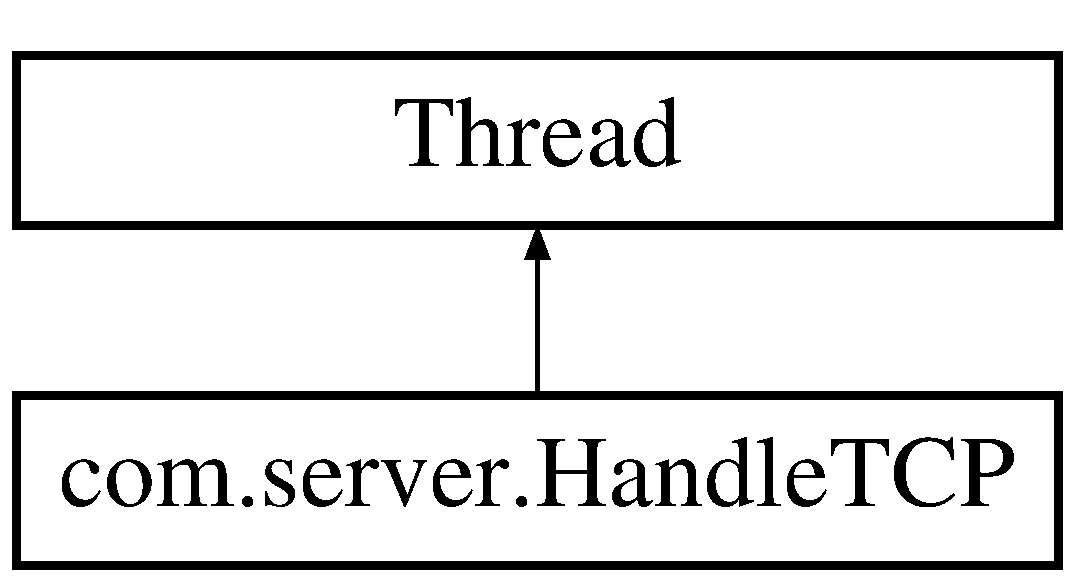
\includegraphics[height=2.000000cm]{classcom_1_1server_1_1HandleTCP}
\end{center}
\end{figure}
\subsection*{Public Member Functions}
\begin{DoxyCompactItemize}
\item 
\hyperlink{classcom_1_1server_1_1HandleTCP_ad94afba7e2974794a5f44015e1c46a4d}{Handle\-T\-C\-P} (Socket client, int which\-Port)
\begin{DoxyCompactList}\small\item\em Constructor for T\-C\-P Handler. \end{DoxyCompactList}\item 
\hypertarget{classcom_1_1server_1_1HandleTCP_a695e48bf0df4e770e89fc8cb1b7a8511}{void \hyperlink{classcom_1_1server_1_1HandleTCP_a695e48bf0df4e770e89fc8cb1b7a8511}{run} ()}\label{classcom_1_1server_1_1HandleTCP_a695e48bf0df4e770e89fc8cb1b7a8511}

\begin{DoxyCompactList}\small\item\em Main method to manage T\-C\-P connections, checks port number and redirects to the appropriate managing method. \end{DoxyCompactList}\end{DoxyCompactItemize}
\subsection*{Private Member Functions}
\begin{DoxyCompactItemize}
\item 
void \hyperlink{classcom_1_1server_1_1HandleTCP_aa9343d9503bbc43f40bab5a0eb309c2b}{data\-Dump} (Data\-Output\-Stream out)  throws I\-O\-Exception 
\begin{DoxyCompactList}\small\item\em Method to dump data onto the calling client Dumps 100\-M\-B of random data. \end{DoxyCompactList}\item 
void \hyperlink{classcom_1_1server_1_1HandleTCP_ab5dfcf570b2f843569c96c2ee461839c}{black\-Hole} (Input\-Stream ins)
\begin{DoxyCompactList}\small\item\em Method provides a dumping ground for data to test upload speeds. \end{DoxyCompactList}\end{DoxyCompactItemize}
\subsection*{Private Attributes}
\begin{DoxyCompactItemize}
\item 
\hypertarget{classcom_1_1server_1_1HandleTCP_a5ecfa869e35d742ad0a43421578ce3f8}{Socket {\bfseries client}}\label{classcom_1_1server_1_1HandleTCP_a5ecfa869e35d742ad0a43421578ce3f8}

\item 
\hypertarget{classcom_1_1server_1_1HandleTCP_aad0c50ffed85d5f4fa3a4c91f893b23a}{final int {\bfseries which\-Port}}\label{classcom_1_1server_1_1HandleTCP_aad0c50ffed85d5f4fa3a4c91f893b23a}

\end{DoxyCompactItemize}
\subsection*{Static Private Attributes}
\begin{DoxyCompactItemize}
\item 
\hypertarget{classcom_1_1server_1_1HandleTCP_ad068267a7062ccee4b5c33cca5c6a42b}{static final int {\bfseries B\-Y\-T\-E\-S\-\_\-\-I\-N\-\_\-\-M\-E\-G\-A\-B\-Y\-T\-E\-S} = 1048576}\label{classcom_1_1server_1_1HandleTCP_ad068267a7062ccee4b5c33cca5c6a42b}

\end{DoxyCompactItemize}


\subsection{Detailed Description}
This class to manage upload and download requests via T\-C\-P. 

\begin{DoxyAuthor}{Author}
Christopher Jordan , William Daniels 
\end{DoxyAuthor}
\begin{DoxyVersion}{Version}
1.\-1 
\end{DoxyVersion}


\subsection{Constructor \& Destructor Documentation}
\hypertarget{classcom_1_1server_1_1HandleTCP_ad94afba7e2974794a5f44015e1c46a4d}{\index{com\-::server\-::\-Handle\-T\-C\-P@{com\-::server\-::\-Handle\-T\-C\-P}!Handle\-T\-C\-P@{Handle\-T\-C\-P}}
\index{Handle\-T\-C\-P@{Handle\-T\-C\-P}!com::server::HandleTCP@{com\-::server\-::\-Handle\-T\-C\-P}}
\subsubsection[{Handle\-T\-C\-P}]{\setlength{\rightskip}{0pt plus 5cm}com.\-server.\-Handle\-T\-C\-P.\-Handle\-T\-C\-P (
\begin{DoxyParamCaption}
\item[{Socket}]{client, }
\item[{int}]{which\-Port}
\end{DoxyParamCaption}
)\hspace{0.3cm}{\ttfamily [inline]}}}\label{classcom_1_1server_1_1HandleTCP_ad94afba7e2974794a5f44015e1c46a4d}


Constructor for T\-C\-P Handler. 


\begin{DoxyParams}{Parameters}
{\em Socket} & \char`\"{}client\char`\"{} for connection \\
\hline
{\em Int} & \char`\"{}which\-Port\char`\"{} for connection \\
\hline
\end{DoxyParams}


\subsection{Member Function Documentation}
\hypertarget{classcom_1_1server_1_1HandleTCP_ab5dfcf570b2f843569c96c2ee461839c}{\index{com\-::server\-::\-Handle\-T\-C\-P@{com\-::server\-::\-Handle\-T\-C\-P}!black\-Hole@{black\-Hole}}
\index{black\-Hole@{black\-Hole}!com::server::HandleTCP@{com\-::server\-::\-Handle\-T\-C\-P}}
\subsubsection[{black\-Hole}]{\setlength{\rightskip}{0pt plus 5cm}void com.\-server.\-Handle\-T\-C\-P.\-black\-Hole (
\begin{DoxyParamCaption}
\item[{Input\-Stream}]{ins}
\end{DoxyParamCaption}
)\hspace{0.3cm}{\ttfamily [inline]}, {\ttfamily [private]}}}\label{classcom_1_1server_1_1HandleTCP_ab5dfcf570b2f843569c96c2ee461839c}


Method provides a dumping ground for data to test upload speeds. 


\begin{DoxyParams}{Parameters}
{\em Input\-Stream} & \char`\"{}ins\char`\"{} provides input stream for data being uploaded \\
\hline
\end{DoxyParams}
\hypertarget{classcom_1_1server_1_1HandleTCP_aa9343d9503bbc43f40bab5a0eb309c2b}{\index{com\-::server\-::\-Handle\-T\-C\-P@{com\-::server\-::\-Handle\-T\-C\-P}!data\-Dump@{data\-Dump}}
\index{data\-Dump@{data\-Dump}!com::server::HandleTCP@{com\-::server\-::\-Handle\-T\-C\-P}}
\subsubsection[{data\-Dump}]{\setlength{\rightskip}{0pt plus 5cm}void com.\-server.\-Handle\-T\-C\-P.\-data\-Dump (
\begin{DoxyParamCaption}
\item[{Data\-Output\-Stream}]{out}
\end{DoxyParamCaption}
) throws I\-O\-Exception\hspace{0.3cm}{\ttfamily [inline]}, {\ttfamily [private]}}}\label{classcom_1_1server_1_1HandleTCP_aa9343d9503bbc43f40bab5a0eb309c2b}


Method to dump data onto the calling client Dumps 100\-M\-B of random data. 


\begin{DoxyParams}{Parameters}
{\em Data\-Output\-Stream} & \char`\"{}out\char`\"{} that provides an outgoing connection to the client. \\
\hline
\end{DoxyParams}

\begin{DoxyExceptions}{Exceptions}
{\em I\-O\-Exception} & to catch any read/write errors. \\
\hline
\end{DoxyExceptions}


The documentation for this class was generated from the following file\-:\begin{DoxyCompactItemize}
\item 
src/main/java/com/server/Handle\-T\-C\-P.\-java\end{DoxyCompactItemize}

\hypertarget{classcom_1_1server_1_1HandleUDP}{\section{com.\-server.\-Handle\-U\-D\-P Class Reference}
\label{classcom_1_1server_1_1HandleUDP}\index{com.\-server.\-Handle\-U\-D\-P@{com.\-server.\-Handle\-U\-D\-P}}
}


This class handles most the primary U\-D\-P Upload and Download functionality for the server.  


\subsection*{Public Member Functions}
\begin{DoxyCompactItemize}
\item 
\hyperlink{classcom_1_1server_1_1HandleUDP_a0b8ef4313d758274df6927dc2e9e2dba}{Handle\-U\-D\-P} (Datagram\-Socket client, int which\-Port)
\begin{DoxyCompactList}\small\item\em constructor for the class, takes two parameters, as well as starts the thread. \end{DoxyCompactList}\item 
\hypertarget{classcom_1_1server_1_1HandleUDP_a321b13bfe67f933e522f7f3d184d9834}{void \hyperlink{classcom_1_1server_1_1HandleUDP_a321b13bfe67f933e522f7f3d184d9834}{run} ()}\label{classcom_1_1server_1_1HandleUDP_a321b13bfe67f933e522f7f3d184d9834}

\begin{DoxyCompactList}\small\item\em simply chooses a port and runs it. \end{DoxyCompactList}\end{DoxyCompactItemize}
\subsection*{Private Member Functions}
\begin{DoxyCompactItemize}
\item 
void \hyperlink{classcom_1_1server_1_1HandleUDP_aa4bfb125e4d66d55fefb7fbe88544d32}{upload\-Black\-Hole} ()
\begin{DoxyCompactList}\small\item\em This method handles all of the upload logic for the U\-D\-P protocol. \end{DoxyCompactList}\item 
\hypertarget{classcom_1_1server_1_1HandleUDP_ab6e9ceefc50e98e285c00dc8999f70e7}{void {\bfseries download\-Data\-Dump} ()}\label{classcom_1_1server_1_1HandleUDP_ab6e9ceefc50e98e285c00dc8999f70e7}

\end{DoxyCompactItemize}
\subsection*{Private Attributes}
\begin{DoxyCompactItemize}
\item 
\hypertarget{classcom_1_1server_1_1HandleUDP_a4dcb0a95b3431a88f398282ec3a499dc}{final Map$<$ String, Time\-Stamp\-Value $>$ {\bfseries address\-Table}}\label{classcom_1_1server_1_1HandleUDP_a4dcb0a95b3431a88f398282ec3a499dc}

\item 
\hypertarget{classcom_1_1server_1_1HandleUDP_ab24c8005f47ea8f5ac71320473946a6f}{final Datagram\-Socket {\bfseries client}}\label{classcom_1_1server_1_1HandleUDP_ab24c8005f47ea8f5ac71320473946a6f}

\item 
\hypertarget{classcom_1_1server_1_1HandleUDP_a34ce0e6d194601f10ea85144d57bd452}{final int {\bfseries which\-Port}}\label{classcom_1_1server_1_1HandleUDP_a34ce0e6d194601f10ea85144d57bd452}

\end{DoxyCompactItemize}
\subsection*{Static Private Attributes}
\begin{DoxyCompactItemize}
\item 
\hypertarget{classcom_1_1server_1_1HandleUDP_af20e767dcb9aebe5f9a691d4c419d885}{static final int {\bfseries O\-N\-E\-\_\-\-M\-I\-N\-U\-T\-E\-\_\-\-I\-N\-\_\-\-M\-I\-L\-L\-I\-S\-E\-C\-O\-N\-D\-S} = 60000}\label{classcom_1_1server_1_1HandleUDP_af20e767dcb9aebe5f9a691d4c419d885}

\item 
\hypertarget{classcom_1_1server_1_1HandleUDP_a0be809a15b91cf0e1218c9a9fe4083dd}{static final int {\bfseries M\-A\-X\-I\-M\-U\-M\-\_\-\-P\-A\-C\-K\-E\-T\-\_\-\-S\-I\-Z\-E} = 30 $\ast$ 1024}\label{classcom_1_1server_1_1HandleUDP_a0be809a15b91cf0e1218c9a9fe4083dd}

\end{DoxyCompactItemize}


\subsection{Detailed Description}
This class handles most the primary U\-D\-P Upload and Download functionality for the server. 

All of the various handling of packets, whether it be dumping or recieving is handled inside. A side note\-: A\-L\-L of the methods used for building the 'willdp' aka\-: the baby protocol on top of U\-D\-P the server uses to specifically consider '0' (that is, the char value of 0), to be the finishing bit for the connection. once that is reached, the respective sender is expected to send, in this order\-: a packet containing the ip\-Address to bind to, as well as a port number.

\begin{DoxyAuthor}{Author}
William Daniels 
\end{DoxyAuthor}
\begin{DoxyVersion}{Version}
1.\-1 
\end{DoxyVersion}


\subsection{Constructor \& Destructor Documentation}
\hypertarget{classcom_1_1server_1_1HandleUDP_a0b8ef4313d758274df6927dc2e9e2dba}{\index{com\-::server\-::\-Handle\-U\-D\-P@{com\-::server\-::\-Handle\-U\-D\-P}!Handle\-U\-D\-P@{Handle\-U\-D\-P}}
\index{Handle\-U\-D\-P@{Handle\-U\-D\-P}!com::server::HandleUDP@{com\-::server\-::\-Handle\-U\-D\-P}}
\subsubsection[{Handle\-U\-D\-P}]{\setlength{\rightskip}{0pt plus 5cm}com.\-server.\-Handle\-U\-D\-P.\-Handle\-U\-D\-P (
\begin{DoxyParamCaption}
\item[{Datagram\-Socket}]{client, }
\item[{int}]{which\-Port}
\end{DoxyParamCaption}
)\hspace{0.3cm}{\ttfamily [inline]}}}\label{classcom_1_1server_1_1HandleUDP_a0b8ef4313d758274df6927dc2e9e2dba}


constructor for the class, takes two parameters, as well as starts the thread. 


\begin{DoxyParams}{Parameters}
{\em client} & The Datagram\-Socket that is connected to. \\
\hline
{\em which\-Port} & an int that tells which port has been passed in. \\
\hline
\end{DoxyParams}


\subsection{Member Function Documentation}
\hypertarget{classcom_1_1server_1_1HandleUDP_aa4bfb125e4d66d55fefb7fbe88544d32}{\index{com\-::server\-::\-Handle\-U\-D\-P@{com\-::server\-::\-Handle\-U\-D\-P}!upload\-Black\-Hole@{upload\-Black\-Hole}}
\index{upload\-Black\-Hole@{upload\-Black\-Hole}!com::server::HandleUDP@{com\-::server\-::\-Handle\-U\-D\-P}}
\subsubsection[{upload\-Black\-Hole}]{\setlength{\rightskip}{0pt plus 5cm}void com.\-server.\-Handle\-U\-D\-P.\-upload\-Black\-Hole (
\begin{DoxyParamCaption}
{}
\end{DoxyParamCaption}
)\hspace{0.3cm}{\ttfamily [inline]}, {\ttfamily [private]}}}\label{classcom_1_1server_1_1HandleUDP_aa4bfb125e4d66d55fefb7fbe88544d32}


This method handles all of the upload logic for the U\-D\-P protocol. 

When a connection is made to it, it 'black holes' all of the given information, and disposes it. It waits until the exit character (0) is sent to it, and then tries to connect to a remote host with the next two packets. 

The documentation for this class was generated from the following file\-:\begin{DoxyCompactItemize}
\item 
src/main/java/com/server/Handle\-U\-D\-P.\-java\end{DoxyCompactItemize}

\hypertarget{classcom_1_1server_1_1Server}{\section{com.\-server.\-Server Class Reference}
\label{classcom_1_1server_1_1Server}\index{com.\-server.\-Server@{com.\-server.\-Server}}
}


This class acts as the basic port handler, and contains the primary server loop.  


\subsection*{Public Member Functions}
\begin{DoxyCompactItemize}
\item 
void \hyperlink{classcom_1_1server_1_1Server_a673471b8c62caeb3e6058293f309da4f}{start\-Server} ()
\begin{DoxyCompactList}\small\item\em This method acts as the main thread starter for the program. \end{DoxyCompactList}\item 
\hypertarget{classcom_1_1server_1_1Server_a534f1955b0d607422970e36f674435ce}{void \hyperlink{classcom_1_1server_1_1Server_a534f1955b0d607422970e36f674435ce}{spinup\-Server\-Socket} (Server\-Socket listen, int udp\-Port)}\label{classcom_1_1server_1_1Server_a534f1955b0d607422970e36f674435ce}

\begin{DoxyCompactList}\small\item\em method spinup\-Server\-Socket This method starts all of the connetions, and listens in a loop to all of them. \end{DoxyCompactList}\end{DoxyCompactItemize}
\subsection*{Static Private Attributes}
\begin{DoxyCompactItemize}
\item 
\hypertarget{classcom_1_1server_1_1Server_a195a2fd46a6d4ed383f37b372acf4a6e}{static final int \hyperlink{classcom_1_1server_1_1Server_a195a2fd46a6d4ed383f37b372acf4a6e}{H\-T\-T\-P\-\_\-\-P\-O\-R\-T} = 3962}\label{classcom_1_1server_1_1Server_a195a2fd46a6d4ed383f37b372acf4a6e}

\begin{DoxyCompactList}\small\item\em http upload and download port \end{DoxyCompactList}\item 
\hypertarget{classcom_1_1server_1_1Server_a667e9966e73c481be93420c2678b5e44}{static final int \hyperlink{classcom_1_1server_1_1Server_a667e9966e73c481be93420c2678b5e44}{U\-D\-P\-\_\-\-U\-P\-L\-O\-A\-D\-\_\-\-P\-O\-R\-T} = 6001}\label{classcom_1_1server_1_1Server_a667e9966e73c481be93420c2678b5e44}

\begin{DoxyCompactList}\small\item\em U\-D\-P Upload port. \end{DoxyCompactList}\item 
\hypertarget{classcom_1_1server_1_1Server_a75ebb782b7f93a00767c42ecc06e948f}{static final int \hyperlink{classcom_1_1server_1_1Server_a75ebb782b7f93a00767c42ecc06e948f}{U\-D\-P\-\_\-\-D\-O\-W\-N\-L\-O\-A\-D\-\_\-\-P\-O\-R\-T} = 9999}\label{classcom_1_1server_1_1Server_a75ebb782b7f93a00767c42ecc06e948f}

\begin{DoxyCompactList}\small\item\em U\-D\-P Download port. \end{DoxyCompactList}\item 
\hypertarget{classcom_1_1server_1_1Server_a2dc0717a250239ef76137e0d76d717a5}{static final int \hyperlink{classcom_1_1server_1_1Server_a2dc0717a250239ef76137e0d76d717a5}{T\-C\-P\-\_\-\-U\-P\-L\-O\-A\-D\-\_\-\-P\-O\-R\-T} = 8080}\label{classcom_1_1server_1_1Server_a2dc0717a250239ef76137e0d76d717a5}

\begin{DoxyCompactList}\small\item\em T\-C\-P Upload port. \end{DoxyCompactList}\item 
\hypertarget{classcom_1_1server_1_1Server_a0a6de32d93cfa5d736a594c1b163a555}{static final int \hyperlink{classcom_1_1server_1_1Server_a0a6de32d93cfa5d736a594c1b163a555}{T\-C\-P\-\_\-\-D\-O\-W\-N\-L\-O\-A\-D\-\_\-\-P\-O\-R\-T} = 8000}\label{classcom_1_1server_1_1Server_a0a6de32d93cfa5d736a594c1b163a555}

\begin{DoxyCompactList}\small\item\em T\-C\-P Downlaod port. \end{DoxyCompactList}\end{DoxyCompactItemize}


\subsection{Detailed Description}
This class acts as the basic port handler, and contains the primary server loop. 

All Port handling, and handing off to threads, essentially happens here.

\begin{DoxyAuthor}{Author}
William Daniels 
\end{DoxyAuthor}
\begin{DoxyVersion}{Version}
1.\-1 
\end{DoxyVersion}


\subsection{Member Function Documentation}
\hypertarget{classcom_1_1server_1_1Server_a673471b8c62caeb3e6058293f309da4f}{\index{com\-::server\-::\-Server@{com\-::server\-::\-Server}!start\-Server@{start\-Server}}
\index{start\-Server@{start\-Server}!com::server::Server@{com\-::server\-::\-Server}}
\subsubsection[{start\-Server}]{\setlength{\rightskip}{0pt plus 5cm}void com.\-server.\-Server.\-start\-Server (
\begin{DoxyParamCaption}
{}
\end{DoxyParamCaption}
)\hspace{0.3cm}{\ttfamily [inline]}}}\label{classcom_1_1server_1_1Server_a673471b8c62caeb3e6058293f309da4f}


This method acts as the main thread starter for the program. 

kicks off all the threads. 

The documentation for this class was generated from the following file\-:\begin{DoxyCompactItemize}
\item 
src/main/java/com/server/Server.\-java\end{DoxyCompactItemize}

\hypertarget{classcom_1_1server_1_1ServerHandler}{\section{com.\-server.\-Server\-Handler Class Reference}
\label{classcom_1_1server_1_1ServerHandler}\index{com.\-server.\-Server\-Handler@{com.\-server.\-Server\-Handler}}
}


This class is the entry point into the program where the main method lives.  


\subsection*{Static Public Member Functions}
\begin{DoxyCompactItemize}
\item 
\hypertarget{classcom_1_1server_1_1ServerHandler_a49b67ff40a33f6094887b9e0cdada70f}{static void {\bfseries main} (String argv\mbox{[}$\,$\mbox{]})}\label{classcom_1_1server_1_1ServerHandler_a49b67ff40a33f6094887b9e0cdada70f}

\end{DoxyCompactItemize}


\subsection{Detailed Description}
This class is the entry point into the program where the main method lives. 

\begin{DoxyAuthor}{Author}
William Daniels 
\end{DoxyAuthor}


The documentation for this class was generated from the following file\-:\begin{DoxyCompactItemize}
\item 
src/main/java/com/server/Server\-Handler.\-java\end{DoxyCompactItemize}

\hypertarget{classcom_1_1server_1_1ServerThread}{\section{com.\-server.\-Server\-Thread Class Reference}
\label{classcom_1_1server_1_1ServerThread}\index{com.\-server.\-Server\-Thread@{com.\-server.\-Server\-Thread}}
}


This class is the class that checks the clients local port, and hands off threads accordingly.  


\subsection*{Public Member Functions}
\begin{DoxyCompactItemize}
\item 
\hypertarget{classcom_1_1server_1_1ServerThread_a7394c023583e8949b69cf664fe61539a}{{\bfseries Server\-Thread} (Socket client)}\label{classcom_1_1server_1_1ServerThread_a7394c023583e8949b69cf664fe61539a}

\item 
\hypertarget{classcom_1_1server_1_1ServerThread_acb48783d33cdc7b6ba983964b75de4a7}{{\bfseries Server\-Thread} (Datagram\-Socket udp\-Client)}\label{classcom_1_1server_1_1ServerThread_acb48783d33cdc7b6ba983964b75de4a7}

\item 
\hypertarget{classcom_1_1server_1_1ServerThread_a27a2a717d36ba29a5e6159ddf2bb8157}{void {\bfseries run} ()}\label{classcom_1_1server_1_1ServerThread_a27a2a717d36ba29a5e6159ddf2bb8157}

\end{DoxyCompactItemize}
\subsection*{Private Member Functions}
\begin{DoxyCompactItemize}
\item 
\hypertarget{classcom_1_1server_1_1ServerThread_a9f2b832582c529244e68717a480e47bf}{void {\bfseries tcp\-Upload} ()}\label{classcom_1_1server_1_1ServerThread_a9f2b832582c529244e68717a480e47bf}

\item 
\hypertarget{classcom_1_1server_1_1ServerThread_ac0e13af4a5f77da90d873e666016317c}{void {\bfseries tcp\-Download} ()}\label{classcom_1_1server_1_1ServerThread_ac0e13af4a5f77da90d873e666016317c}

\item 
\hypertarget{classcom_1_1server_1_1ServerThread_ab3bfacb3d82a51db195ecfef733f2ea1}{void {\bfseries udp\-Upload} ()}\label{classcom_1_1server_1_1ServerThread_ab3bfacb3d82a51db195ecfef733f2ea1}

\item 
\hypertarget{classcom_1_1server_1_1ServerThread_a69d6ff48a1d14da7d40968d5b3a1d2cb}{void {\bfseries udp\-Download} ()}\label{classcom_1_1server_1_1ServerThread_a69d6ff48a1d14da7d40968d5b3a1d2cb}

\item 
\hypertarget{classcom_1_1server_1_1ServerThread_ac9197dc3ac9e06be7fcbdbc72eed7439}{void {\bfseries http\-Handler} ()}\label{classcom_1_1server_1_1ServerThread_ac9197dc3ac9e06be7fcbdbc72eed7439}

\end{DoxyCompactItemize}
\subsection*{Private Attributes}
\begin{DoxyCompactItemize}
\item 
\hypertarget{classcom_1_1server_1_1ServerThread_acdc12e0a8fd08b1c6fc78a8776141cb2}{boolean {\bfseries continue\-U\-D\-P} = true}\label{classcom_1_1server_1_1ServerThread_acdc12e0a8fd08b1c6fc78a8776141cb2}

\item 
\hypertarget{classcom_1_1server_1_1ServerThread_a35497d54ac05820a80b8b6095a5276e8}{Socket {\bfseries client}}\label{classcom_1_1server_1_1ServerThread_a35497d54ac05820a80b8b6095a5276e8}

\item 
\hypertarget{classcom_1_1server_1_1ServerThread_a235f27cd5c41e5bf3a6e341ba54eefc3}{Datagram\-Socket {\bfseries udp\-Client} = null}\label{classcom_1_1server_1_1ServerThread_a235f27cd5c41e5bf3a6e341ba54eefc3}

\end{DoxyCompactItemize}


\subsection{Detailed Description}
This class is the class that checks the clients local port, and hands off threads accordingly. 

\begin{DoxyAuthor}{Author}
William Daniels 
\end{DoxyAuthor}
\begin{DoxyVersion}{Version}
1.\-1 
\end{DoxyVersion}


The documentation for this class was generated from the following file\-:\begin{DoxyCompactItemize}
\item 
src/main/java/com/server/Server\-Thread.\-java\end{DoxyCompactItemize}

%--- End generated contents ---

% Index
\newpage
\phantomsection
\addcontentsline{toc}{part}{Index}
\printindex

\end{document}
